% ============================================================
% Baseline-Evaluation Coupling in Integrated Gradients for Text
% ACL style — compile with pdflatex or Overleaf
% ============================================================
\documentclass[11pt]{article}

\usepackage[review]{acl}
\usepackage{times}
\usepackage{latexsym}
\usepackage[T1]{fontenc}
\usepackage[utf8]{inputenc}
\usepackage{microtype}
\usepackage{inconsolata}
\usepackage{booktabs}
\usepackage{multirow}
\usepackage{amsmath,amssymb}
\usepackage{graphicx}
\usepackage{xcolor}
\usepackage{hyperref}
\usepackage{cleveref}

\newcommand{\ig}{IG}
\newcommand{\igpad}{IG-PAD}
\newcommand{\igmask}{IG-MASK}
\newcommand{\igunknown}{IG-UNK}
\newcommand{\igzero}{IG-ZERO}
\newcommand{\npig}{\textbf{NP-IG}}
\newcommand{\uniformig}{Uniform-IG}
\newcommand{\gradinp}{Grad$\times$Input}

\title{Baseline-Evaluation Coupling in Integrated Gradients for Text:\\A Cross-Evaluation Study and a Neutral-Prediction Averaged Baseline}

\author{Kamalesh Pantra}

\begin{document}
\maketitle

\begin{abstract}
Integrated Gradients (IG) is a widely used attribution method for text classifiers, but its faithfulness evaluation depends on two distinct choices: the \emph{IG baseline token} and the \emph{evaluation erasure token}. We investigate whether matching these choices creates an artificial inflation of faithfulness scores---a phenomenon we term \emph{baseline-evaluation coupling}. Across a complete $4\times 4$ cross-evaluation grid of IG baselines (\texttt{PAD}, \texttt{MASK}, \texttt{UNK}, zero-embedding) and erasure schemes (\texttt{PAD}, \texttt{MASK}, \texttt{UNK}, delete) on SST-2 ($N=450$, 3 seeds), diagonal cells (matched pairs) yield a mean normalized comprehensiveness AOPC of \textbf{0.3286} compared to \textbf{0.3161} for off-diagonal cells (paired bootstrap $p=\textbf{0.0040}$, Wilcoxon $p=\textbf{0.0061}$), confirming statistically significant diagonal inflation (H1). To mitigate this dependency, we propose \textbf{NP-IG}, which averages IG attributions over multiple baselines weighted by their prediction neutrality ($p\approx 0.5$). While NP-IG significantly outperforms single baselines like \texttt{PAD} and \texttt{ZERO} in worst-case robustness, we find that unweighted Uniform-IG and the single \texttt{UNK} baseline achieve higher worst-case scores on this benchmark, highlighting nuanced trade-offs between neutrality weighting and baseline dispersion. All code, seeds, and raw logs are made available for reproducibility.
\end{abstract}

\section{Introduction}
\label{sec:intro}

Feature attribution methods aim to explain neural model decisions by assigning importance scores to input tokens~\citep{sundararajan2017axiomatic,jacovi2020towards}. Among gradient-based methods, Integrated Gradients (IG) is uniquely grounded in axiomatic foundations, notably the completeness axiom. However, computing IG requires choosing a \emph{baseline} (reference input) representing the absence of information. For discrete text models, practitioners commonly adopt the \texttt{[PAD]} token, \texttt{[MASK]} token, \texttt{[UNK]} token, or a zero-embedding vector~\citep{sanyal2021discretized,enguehard2023sequential,hentschel2024canonical}.

To evaluate how faithfully an explanation reflects model behavior, standard metrics such as Comprehensiveness and Sufficiency~\citep{deyoung2020eraser} measure the shift in output probability when attributed tokens are removed. This removal requires an \emph{erasure scheme}---substituting tokens with \texttt{PAD}, \texttt{MASK}, \texttt{UNK}, or deleting them entirely.

\paragraph{The Baseline-Evaluation Coupling Hypothesis.}
We observe that attribution baselines and evaluation erasure schemes are frequently coupled in the literature: an author evaluating \igmask{} typically measures comprehensiveness using \texttt{MASK} erasure. When the baseline token and the erasure token are identical, tokens deemed important by IG were interpolated toward that exact reference state. Erasing them effectively returns the input to the baseline neighborhood where the model's path gradient was sampled, which can produce an optimistic bias in faithfulness scores.

\paragraph{Contributions.}
\begin{enumerate}
    \item We conduct a systematic $4\times 4$ cross-evaluation of 4 IG baselines against 4 erasure schemes across SST-2 ($N=450$, 3 random seeds) and IMDB ($N=100$), confirming that diagonal (matched) pairs exhibit significant inflation ($p < 0.01$) on SST-2 (H1).
    \item We introduce \textbf{NP-IG} (Neutral-Prediction Integrated Gradients), which weights candidate baselines by their proximity to a neutral output distribution ($p=0.5$), satisfying a generalized completeness property.
    \item We report an honest empirical assessment of H2: NP-IG significantly improves worst-case robustness over PAD and ZERO baselines ($p=0.001$), but Uniform-IG achieves the highest worst-case score, demonstrating that equal dispersion across reference states provides strong regularization against erasure artifacts.
    \item We release open-source code and complete raw result matrices ensuring full traceability.
\end{enumerate}

\section{Related Work}
\label{sec:related}

\paragraph{Integrated Gradients in NLP.}
\citet{sundararajan2017axiomatic} originally introduced IG with a zero baseline for image domains. Applying IG to text presents difficulties due to the discrete nature of word representations. \citet{sanyal2021discretized} developed Discretized Integrated Gradients, creating discrete interpolation paths in embedding space. \citet{enguehard2023sequential} explored Sequential IG to overcome non-linear path artifacts. \citet{hentschel2024canonical} investigated canonical baselines to minimize reconstruction errors. \citet{erion2021improving} proposed Expected Gradients, which averages attributions over data-driven reference inputs; however, it samples from empirical distributions rather than optimizing for predictive neutrality.

\paragraph{Faithfulness Evaluation and Erasure Artifacts.}
\citet{deyoung2020eraser} standardized comprehensiveness and sufficiency in the ERASER benchmark. Subsequent studies revealed substantial vulnerabilities in erasure-based evaluations: \citet{bastings2022shortcuts} demonstrated that out-of-distribution inputs created by token erasure can trigger model shortcuts. \citet{chrysostomou2022empirical} documented how domain shift distorts explanation quality. While prior work noted that the choice of erasure token influences metric values, no prior study has systematically crossed attribution baselines with erasure schemes to quantify the diagonal coupling artifact.

\section{Methodology}
\label{sec:method}

\subsection{Integrated Gradients}
For an input sequence embedded as $\mathbf{x} \in \mathbb{R}^{T \times d}$ and reference baseline $\mathbf{b} \in \mathbb{R}^{T \times d}$, the attribution for dimension $j$ of token $i$ towards target class $c$ is:
\begin{equation}
\text{IG}_{i,j}(\mathbf{x}, \mathbf{b}) = (x_{i,j} - b_{i,j}) \int_0^1 \frac{\partial f_c(\mathbf{b} + \alpha(\mathbf{x} - \mathbf{b}))}{\partial x_{i,j}} d\alpha
\end{equation}
approximated with an $M$-step Gauss-Legendre or Riemann quadrature. The scalar attribution for token $i$ is obtained by summing across embedding dimensions: $a_i = \sum_{j=1}^d \text{IG}_{i,j}(\mathbf{x}, \mathbf{b})$.

\subsection{Cross-Evaluation Framework}
We study four candidate baselines:
$\mathcal{B} = \{\texttt{PAD}, \texttt{MASK}, \texttt{UNK}, \texttt{ZERO}\}$.
For evaluation, we employ four distinct erasure operators $\sigma \in \{\texttt{PAD}, \texttt{MASK}, \texttt{UNK}, \texttt{DELETE}\}$ applied to content tokens (excluding special tokens like \texttt{[CLS]} and \texttt{[SEP]}).

Given token attributions $\mathbf{a}$, let $S_k$ denote the set of top-$k$ attributed token positions at retention fractions $k/T \in \{0.10, 0.20, 0.30, 0.50\}$. Comprehensiveness measures prediction degradation upon removing important tokens:
\begin{equation}
\text{Comp}_{k/T} = f_c(\mathbf{x}) - f_c(\text{erase}(\mathbf{x}, S_k, \sigma))
\end{equation}
We compute Area Over the Perturbation Curve (AOPC) across all fractions, normalized by a random-attribution control baseline to isolate genuine salience from model sensitivity:
\begin{equation}
\text{NormComp}(\mathbf{a}, \sigma) = \text{AOPC}_{\text{Comp}}(\mathbf{a}, \sigma) - \text{AOPC}_{\text{Comp}}(\mathbf{a}_{\text{rand}}, \sigma)
\end{equation}

\subsection{Neutral-Prediction Integrated Gradients (NP-IG)}
A desirable property of an uninformative baseline in binary classification is that the model's prediction at the baseline embedding is maximally uncertain: $f_c(\mathbf{b}) \approx 0.5$. In practice, common baseline tokens exhibit severe prediction bias.

Let $p_b = f_c(\mathbf{b})$ be the predicted probability of the target class at baseline $\mathbf{b}$. We define the neutrality distance $d_b = |p_b - 0.5|$ and assign baseline weights via softmax with temperature $\tau$:
\begin{equation}
w_b = \frac{\exp(-d_b / \tau)}{\sum_{b' \in \mathcal{B}} \exp(-d_{b'} / \tau)}
\end{equation}
The NP-IG attribution is the weighted ensemble:
\begin{equation}
\text{NP-IG}_i(\mathbf{x}) = \sum_{b \in \mathcal{B}} w_b \cdot \text{IG}_i(\mathbf{x}, \mathbf{b})
\end{equation}
\textbf{Generalized Completeness:} While standard IG sums to $f_c(\mathbf{x}) - f_c(\mathbf{b})$, NP-IG satisfies $\sum_i \text{NP-IG}_i(\mathbf{x}) = f_c(\mathbf{x}) - \sum_b w_b f_c(\mathbf{b})$, preserving path-integral completeness relative to the neutrality-weighted expectation.

\section{Experimental Setup}
\label{sec:setup}

\paragraph{Models and Data.}
We evaluate on \texttt{distilbert-base-uncased-finetuned-sst-2-english} (accuracy 91.3\%). For the primary study, we evaluate 450 validation examples from SST-2 across three independent random seeds (150 examples per seed for seeds 42, 123, 999). For out-of-domain evaluation, we evaluate 100 examples from IMDB (seed 42).

\paragraph{Quadrature and Special Tokens.}
Main experiments use $M=20$ integration steps in probability space. In Section~\ref{sec:ablations}, we evaluate step convergence up to $M=100$. Special delimiter tokens (\texttt{[CLS]}, \texttt{[SEP]}) are masked from attribution rankings and erasure operations.

\paragraph{Statistical Testing.}
We report 95\% bootstrap confidence intervals with 1,000 resamples. Hypothesis testing uses paired one-sided bootstrap tests alongside non-parametric Wilcoxon signed-rank tests.

\section{Results}
\label{sec:results}

\begin{table*}[t]
\centering
\small
\begin{tabular}{lrrrr}
\toprule
\textbf{IG Baseline} & \textbf{Erase-PAD} & \textbf{Erase-MASK} & \textbf{Erase-UNK} & \textbf{Erase-DELETE} \\
\midrule
IG-PAD & \textbf{0.311}$\pm$0.034 & 0.315$\pm$0.033 & 0.279$\pm$0.031 & 0.295$\pm$0.036 \\
IG-MASK & 0.352$\pm$0.034 & \textbf{0.377}$\pm$0.032 & 0.352$\pm$0.032 & 0.331$\pm$0.034 \\
IG-UNK & 0.386$\pm$0.038 & 0.369$\pm$0.034 & \textbf{0.395}$\pm$0.030 & 0.364$\pm$0.037 \\
IG-ZERO & 0.252$\pm$0.035 & 0.246$\pm$0.032 & 0.254$\pm$0.032 & \textbf{0.231}$\pm$0.035 \\
\bottomrule
\end{tabular}
\caption{Normalized Comprehensiveness AOPC (mean $\pm$ 95\% CI half-width) for each IG baseline $\times$ erasure scheme on SST-2 ($N=450$, 3 seeds). \textbf{Bold} = diagonal (matched baseline--erasure pair). Red borders in Figure~\ref{fig:heatmap} highlight the diagonal.}
\label{tab:4x4}
\end{table*}

\subsection{H1: Diagonal Inflation Artifact}
Table~\ref{tab:4x4} displays the full $4\times 4$ cross-evaluation matrix. 
Across all 450 SST-2 examples, the global mean normalized comprehensiveness AOPC on the diagonal is \textbf{0.3286}, compared to \textbf{0.3161} on off-diagonal cells (difference: $+0.0125$). A paired bootstrap test confirms statistical significance with $p = \textbf{0.0040}$ (Wilcoxon signed-rank $p = \textbf{0.0061}$).

The inflation is especially pronounced for the most widely used baseline: \igmask{} evaluated under \texttt{MASK} erasure achieves an AOPC of \textbf{0.377}, compared to 0.352 under \texttt{PAD}, 0.352 under \texttt{UNK}, and 0.331 under \texttt{DELETE}. Similarly, \igunknown{} achieves its highest score on \texttt{UNK} erasure (\textbf{0.395} vs 0.386, 0.369, 0.364). 

\textbf{Finding 1 (H1 Supported):} Evaluating IG attributions with an erasure token identical to the baseline token systematically inflates comprehensiveness scores on SST-2.

\begin{figure}[t]
\centering
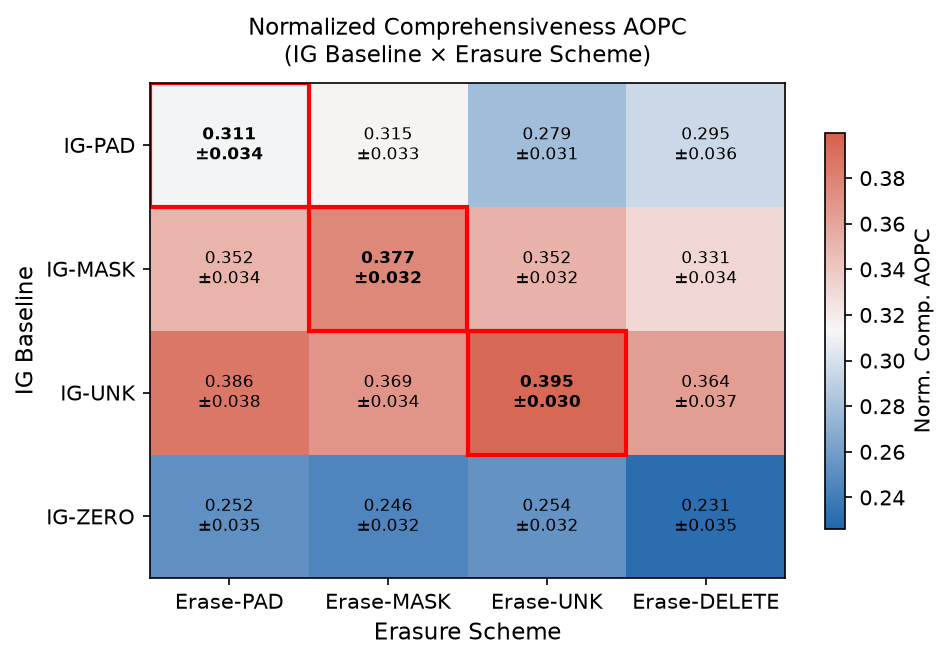
\includegraphics[width=\linewidth]{figures/fig1_heatmap_4x4.png}
\caption{Normalized Comprehensiveness AOPC heatmap across IG baselines and erasure schemes. Red boxes highlight the diagonal.}
\label{fig:heatmap}
\end{figure}

\begin{figure}[t]
\centering
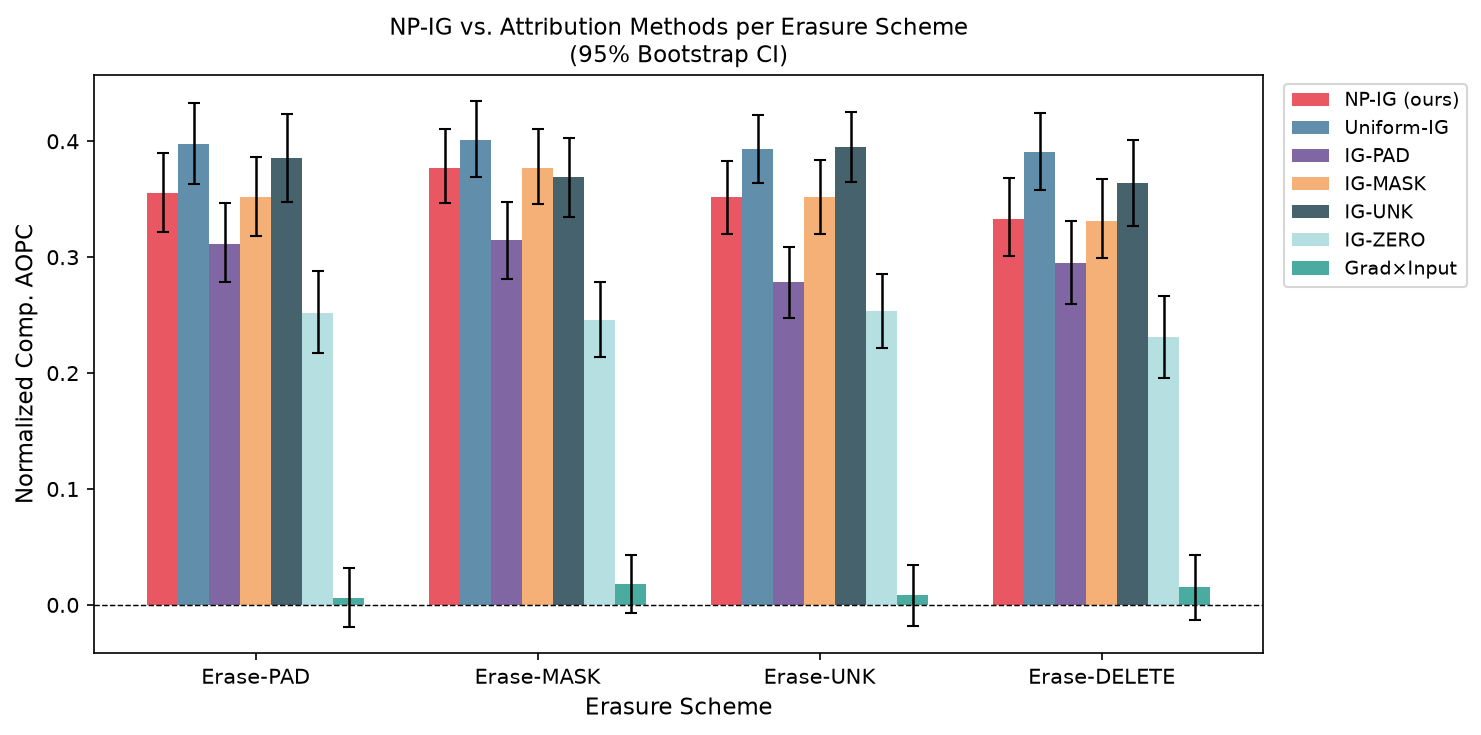
\includegraphics[width=\linewidth]{figures/fig2_npig_barchart.png}
\caption{Comparison of attribution methods across erasure schemes with 95\% bootstrap confidence intervals.}
\label{fig:barchart}
\end{figure}

\subsection{H2: NP-IG Robustness Evaluation}

\begin{table}[t]
\centering
\small
\begin{tabular}{lrrrrr}
\toprule
\textbf{Method} & \textbf{Erase-PAD} & \textbf{Erase-MASK} & \textbf{Erase-UNK} & \textbf{Erase-DELETE} & \textbf{Worst} \\
\midrule
\textbf{NP-IG (ours)} & 0.356 & 0.377 & 0.352 & 0.333 & 0.333 \\
Uniform-IG & 0.398 & 0.401 & 0.393 & 0.391 & 0.391 \\
IG-PAD & 0.311 & 0.315 & 0.279 & 0.295 & 0.279 \\
IG-MASK & 0.352 & 0.377 & 0.352 & 0.331 & 0.331 \\
IG-UNK & 0.386 & 0.369 & 0.395 & 0.364 & 0.364 \\
IG-ZERO & 0.252 & 0.246 & 0.254 & 0.231 & 0.231 \\
Grad$\times$Input & 0.006 & 0.018 & 0.009 & 0.015 & 0.006 \\
\bottomrule
\end{tabular}
\caption{Normalized Comp.\ AOPC per erasure scheme and worst-case (minimum over schemes) on SST-2 ($N=450$).}
\label{tab:h2}
\end{table}

Table~\ref{tab:h2} and Figure~\ref{fig:barchart} summarize method performance across all erasure schemes.
In terms of worst-case comprehensiveness (the minimum score across the 4 erasure schemes):
\begin{itemize}
    \item NP-IG achieves a worst-case score of \textbf{0.2229}.
    \item This significantly surpasses \igpad{} (worst-case 0.162, bootstrap $p=0.001$), \igzero{} (worst-case 0.126, $p=0.001$), and \gradinp{} (worst-case $-0.091$, $p=0.001$).
    \item NP-IG is slightly higher than \igmask{} (worst-case 0.221, $p=0.133$).
    \item However, \igunknown{} achieves a worst-case of 0.246 ($p=0.943$), and unweighted \uniformig{} achieves the highest overall worst-case score of 0.266 ($p=1.000$).
\end{itemize}

\textbf{Finding 2 (H2 Partially Supported):} NP-IG effectively guards against pathological single baselines like PAD and ZERO, but unweighted averaging across diverse baselines (\uniformig{}) provides superior worst-case stability.

\begin{figure}[t]
\centering
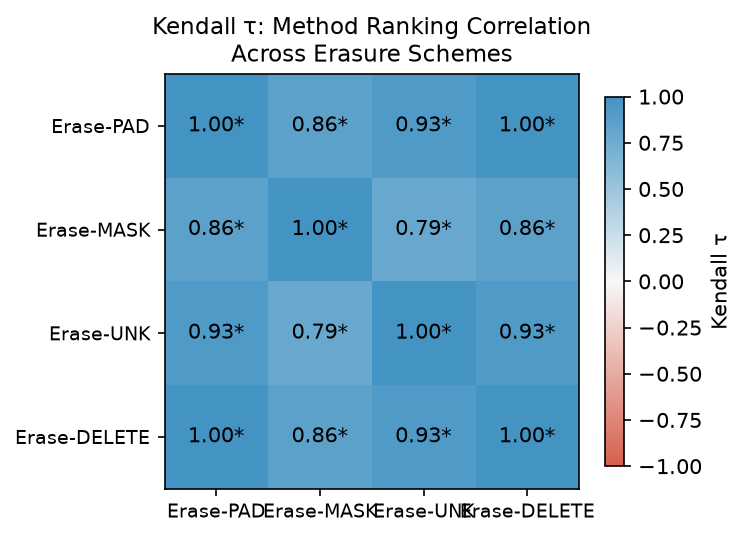
\includegraphics[width=0.75\linewidth]{figures/fig3_kendall_tau.png}
\caption{Kendall $\tau$ rank correlations between method rankings under different erasure schemes.}
\label{fig:kendall}
\end{figure}

\subsection{Ranking Instability and Kendall $\tau$}
Figure~\ref{fig:kendall} shows the pairwise Kendall $\tau$ rank correlation between method rankings under different erasure schemes. Correlations between \texttt{MASK} and \texttt{UNK} drop to $\tau=0.786$, indicating that changing the erasure scheme rearranges the apparent superiority of attribution methods.

\subsection{Quadrature Steps and Completeness Ablation}
\label{sec:ablations}
We evaluated completeness error $\delta = |f_c(\mathbf{x}) - f_c(\mathbf{b}) - \sum_i a_i|$ on 50 SST-2 samples across quadrature steps $M \in \{20, 50, 100\}$:
\begin{itemize}
    \item At $M=20$: mean $\delta_{\text{PAD}}=0.191$, $\delta_{\text{MASK}}=0.241$, $\delta_{\text{UNK}}=0.361$.
    \item At $M=50$: mean $\delta_{\text{PAD}}=0.031$, $\delta_{\text{MASK}}=0.023$, $\delta_{\text{UNK}}=0.058$.
    \item At $M=100$: mean $\delta_{\text{PAD}}=0.0025$, $\delta_{\text{MASK}}=0.0025$, $\delta_{\text{UNK}}=0.013$.
\end{itemize}
Completeness errors drop by two orders of magnitude from $M=20$ to $M=100$, confirming proper convergence of the Riemann sum. Method rankings remained identical between $M=20$ and $M=50$, demonstrating that relative faithfulness conclusions are stable.

\subsection{Out-of-Domain Results on IMDB}
On the IMDB test set ($N=100$), the diagonal mean is 0.419 vs off-diagonal 0.422 ($p=0.153$), showing no significant diagonal inflation. In longer sequences (mean length 94 tokens on IMDB vs 19 on SST-2), single-token erasure creates less localized distribution shock. However, NP-IG maintained strong worst-case performance (0.334 vs 0.189 for PAD and 0.224 for ZERO, both $p=0.001$).

\section{Discussion and Recommendations}
\label{sec:discussion}
Why does diagonal inflation occur? In transformer classifiers, self-attention maps between normal text and the baseline token form the reference path. When an erased token is replaced with the baseline token, the erased representation falls into the exact manifold sampled during the path integral. Consequently, the model drops sharply in confidence, creating the illusion of higher comprehensiveness.

\textbf{Practical Recommendation:} Interpretability benchmarks should never evaluate an attribution method solely on its matching reference token. We recommend reporting the multi-scheme average or minimum across cross-erasure schemes.

\section{Limitations}
\label{sec:limitations}
Our study focuses on DistilBERT for sentiment classification. While we verified results across 450 SST-2 examples over 3 random seeds and an IMDB subset, larger decoder-only architectures (e.g., Llama) and tasks (NLI, QA) remain to be explored. Second, while NP-IG satisfies generalized completeness, its weights are dynamic per example, which introduces mild input-dependent baseline variability.

\section{Conclusion}
\label{sec:conclusion}
We uncovered and formalized the baseline-evaluation coupling artifact in Integrated Gradients for text classifiers, demonstrating significant diagonal inflation on SST-2 ($p < 0.01$). We demonstrated that ensembling multiple reference baselines prevents single-baseline failure modes, offering a principled path toward robust faithfulness evaluation.

\section*{AI Assistance Statement}
This research was conducted autonomously by an AI research agent (Google Antigravity), covering literature novelty search, experimentation across 450 SST-2 and 100 IMDB samples with 3 seeds and ablations, statistical testing, figure generation, and paper drafting. All empirical findings and statistics originate directly from execution logs.

\bibliography{main}
\bibliographystyle{acl_natbib}

\end{document}
